% =====================================================================
%  Firefly: Problem Proof
%  ---------------------------------------------------------------------
%  Build:   xelatex firefly-problem-proof.tex   (run twice, so the
%           placeholder count on the cover is right)
%           XeLaTeX uses Charter + Avenir Next from macOS when present.
%           pdfLaTeX (e.g. Overleaf's default) uses Charter + Helvetica,
%           which need a full TeX Live; BasicTeX lacks them.
%
%  HOW TO FINISH THIS DOCUMENT
%  1. Every \fillin{...} is a highlighted blank for first-party evidence
%     that does not exist in the repo yet. Replace each one with the real
%     value. The cover shows how many are still open; it must read zero
%     before you submit (the draft banner then disappears by itself).
%  2. Screenshots: save redacted PNG/JPG/PDF files into ./exhibits/ with
%     the file names used in \exhibit{...} below. A dashed frame shows
%     until the file exists. Follow the redaction protocol (Appendix B).
%  3. Never invent numbers, quotes or commitments. If a count is zero,
%     write zero. PRODUCT.md, "Evidence on Hand", applies here too.
%  4. Redacted screenshots of real people are sensitive: think twice
%     before committing ./exhibits/ to the repository.
% =====================================================================

\documentclass[11pt,letterpaper]{article}

% ---------- Fonts: XeLaTeX/LuaLaTeX or pdfLaTeX ----------
% Body: Charter. Headings and data: Avenir Next, else Helvetica.
\usepackage{iftex}
\usepackage{amssymb}
\ifPDFTeX
  \usepackage[T1]{fontenc}
  \usepackage[utf8]{inputenc}
  \usepackage{charter}
  \usepackage[scaled=0.92]{helvet}
\else
  \usepackage{fontspec}
  \IfFontExistsTF{Charter}{\setmainfont{Charter}}{%
    \IfFontExistsTF{XCharter}{\setmainfont{XCharter}}{}}
  \IfFontExistsTF{Avenir Next}{%
    \setsansfont{Avenir Next}[Scale=0.94,BoldFont={Avenir Next Demi Bold}]}{%
    \IfFontExistsTF{Helvetica Neue}{\setsansfont{Helvetica Neue}[Scale=0.94]}{%
      \IfFontExistsTF{TeX Gyre Heros}{\setsansfont{TeX Gyre Heros}[Scale=0.92]}{}}}
\fi
\usepackage{microtype}

% ---------- Layout ----------
\usepackage[letterpaper,top=0.95in,bottom=0.95in,left=1in,right=1in,
            headheight=14pt,headsep=22pt,footskip=34pt]{geometry}
\usepackage{xcolor}
\usepackage{graphicx}
\usepackage{array,tabularx,booktabs,colortbl,longtable}
\usepackage{tikz}
\usepackage{fancyhdr}
\usepackage{etoolbox}
\usepackage{calc}
\usepackage[hidelinks]{hyperref}

\setlength{\parindent}{0pt}
\setlength{\parskip}{6pt}
\linespread{1.08}
\renewcommand{\arraystretch}{1.28}
\setlength{\tabcolsep}{6pt}
\emergencystretch=1.5em

% ---------- Brand palette, adapted for paper ----------
% Glow #D9F84A is the one light: used only as a fill behind dark text or
% as a rule, never as text on white (contrast is too low).
\definecolor{ink}{HTML}{141412}
\definecolor{muted}{HTML}{66665F}
\definecolor{hair}{HTML}{DADAD2}
\definecolor{paper}{HTML}{F5F5F0}
\definecolor{glow}{HTML}{D9F84A}
\definecolor{glowsoft}{HTML}{F1FAC4}
\definecolor{dusk}{HTML}{C3A0FF}
\definecolor{duskdeep}{HTML}{5A3E9E}  % text-safe violet for labels
\definecolor{dusksoft}{HTML}{F1EAFF}
\definecolor{night}{HTML}{050505}
\color{ink}

\hypersetup{
  pdftitle={Firefly: Problem Proof},
  pdfsubject={Customer discovery evidence for Firefly, Vancouver},
  pdfkeywords={Firefly, problem proof, customer discovery, Vancouver},
}

% ---------- Placeholder machinery ----------
\makeatletter
\newcounter{blanks}
\newcommand{\fillin}[2][\footnotesize]{%
  \stepcounter{blanks}%
  {\setlength{\fboxsep}{1.6pt}\colorbox{glow}{\strut\sffamily#1\bfseries\textcolor{night}{#2}}}}
\providecommand{\totalblanks}{0}
\AtEndDocument{\immediate\write\@auxout{\gdef\string\totalblanks{\theblanks}}}
\makeatother

% ---------- Evidence-type tags ----------
\newcommand{\tagbox}[3]{{\setlength{\fboxsep}{2pt}\colorbox{#1}{\sffamily\scriptsize\bfseries\textcolor{#2}{\MakeUppercase{#3}}}}}
\newcommand{\desk}{\tagbox{dusksoft}{duskdeep}{Desk research}}
\newcommand{\firstparty}{\tagbox{glow}{night}{First-party}}
\newcommand{\target}{\tagbox{paper}{muted}{Target, not a result}}
\newcommand{\open}{\tagbox{glow}{night}{Open}}
\newcommand{\done}{\tagbox{dusksoft}{duskdeep}{Done}}

% ---------- Section styling ----------
\makeatletter
\renewcommand{\@seccntformat}[1]{%
  \ifstrequal{#1}{section}{%
    {\color{duskdeep}\sffamily\bfseries\ifnum\value{section}<10 0\fi\thesection}\hspace{0.75em}}{%
    {\color{muted}\csname the#1\endcsname}\hspace{0.6em}}}
\newcommand{\condbreak}[1]{\par\vskip 0pt plus #1\penalty-200\vskip 0pt plus -#1\relax}
\renewcommand{\section}{\condbreak{2.6in}\@startsection{section}{1}{0pt}%
  {-26pt plus -4pt minus -2pt}{10pt}%
  {\sffamily\Large\bfseries\color{ink}}}
\renewcommand{\subsection}{\condbreak{1.5in}\@startsection{subsection}{2}{0pt}%
  {-16pt plus -3pt minus -2pt}{4pt}%
  {\sffamily\normalsize\bfseries\color{ink}}}
\renewcommand{\thesubsection}{\thesection.\arabic{subsection}}
\makeatother

\newcommand{\eyebrow}[1]{{\sffamily\scriptsize\bfseries\color{duskdeep}\MakeUppercase{#1}}\par\vspace{-2pt}}
\newcommand{\lede}[1]{{\large\color{ink}#1}\par}
\newcommand{\src}[1]{{\sffamily\scriptsize\color{muted}#1}}
\newcommand{\colhead}[1]{{\sffamily\footnotesize\bfseries\color{muted}#1}}
\newcommand{\num}[1]{{\sffamily\bfseries #1}}

% ---------- Tight lists (no enumitem needed) ----------
\newenvironment{points}{%
  \begin{list}{\textcolor{duskdeep}{\small$\blacktriangleright$}}{%
    \setlength{\leftmargin}{1.25em}\setlength{\labelwidth}{1em}%
    \setlength{\labelsep}{0.45em}\setlength{\itemsep}{2pt}%
    \setlength{\topsep}{2pt}\setlength{\parsep}{0pt}}}%
  {\end{list}}
\newcounter{stepno}
\newenvironment{steps}{%
  \begin{list}{\sffamily\bfseries\color{duskdeep}\arabic{stepno}.}{%
    \usecounter{stepno}\setlength{\leftmargin}{1.5em}\setlength{\labelwidth}{1.2em}%
    \setlength{\labelsep}{0.4em}\setlength{\itemsep}{2pt}%
    \setlength{\topsep}{2pt}\setlength{\parsep}{0pt}}}%
  {\end{list}}

% ---------- Callout box (left rule, tinted ground) ----------
\newsavebox{\calloutbox}
\newenvironment{callout}[2][glow]{%
  \def\calloutcolor{#1}\def\callouttitle{#2}%
  \begin{lrbox}{\calloutbox}\begin{minipage}{\linewidth-28pt}\setlength{\parskip}{4pt}%
  \ifx\callouttitle\empty\else{\sffamily\small\bfseries\callouttitle}\par\fi}%
  {\end{minipage}\end{lrbox}%
  \par\smallskip\noindent
\begin{tikzpicture}
    \node[fill=paper,inner xsep=12pt,inner ysep=10pt,anchor=north west] (b) at (0,0) {\usebox{\calloutbox}};
    \fill[\calloutcolor] (b.north west) rectangle ([xshift=3.5pt]b.south west);
  \end{tikzpicture}\par\smallskip}

% ---------- Pull quote ----------
\newcommand{\pullquote}[2]{%
  \par\smallskip\noindent\begin{minipage}{\linewidth}
  \hspace*{1.2em}\begin{minipage}{\linewidth-1.2em}
  {\itshape\large ``#1''}\par\vspace{3pt}
  \src{#2}
  \end{minipage}\end{minipage}\par\smallskip}

% ---------- Stat tile ----------
\newcommand{\stat}[4][ink]{% [colour] {number} {label} {source}
  \begin{minipage}[t]{\linewidth}\raggedright
    {\sffamily\bfseries\fontsize{26}{28}\selectfont\color{#1}#2}\par\vspace{2pt}
    {\color{glow}\rule{2.2em}{2.5pt}}\par\vspace{3pt}
    {\small #3}\par\vspace{2pt}
    \src{#4}
  \end{minipage}}

% ---------- Exhibit: screenshot or a labelled empty frame ----------
\newcounter{exhibit}
\renewcommand{\theexhibit}{\Alph{exhibit}}
\newcommand{\exhibit}[4]{% {file} {title} {what goes here} {height}
  \refstepcounter{exhibit}%
  \par\medskip\noindent
  \begin{minipage}{\linewidth}
  {\sffamily\small\bfseries\color{duskdeep}Exhibit \theexhibit\quad\color{ink}#2}\par\vspace{4pt}
  \IfFileExists{exhibits/#1}{%
    \centering\includegraphics[width=\linewidth,height=#4,keepaspectratio]{exhibits/#1}%
  }{%
    \stepcounter{blanks}%
    \begin{tikzpicture}
      \draw[hair,line width=1pt,dashed,fill=paper,rounded corners=3pt] (0.5pt,0.5pt) rectangle (\linewidth-0.5pt,#4-0.5pt);
      \node[text width=\linewidth-1.6in,align=center,font=\sffamily\small] at (0.5\linewidth,0.5*#4)
        {{\setlength{\fboxsep}{2pt}\colorbox{glow}{\bfseries\footnotesize\textcolor{night}{EXHIBIT TO ADD}}}\\[6pt]
         \color{muted}#3\\[4pt]\scriptsize Save as \texttt{exhibits/#1}};
    \end{tikzpicture}%
  }
  \end{minipage}\par\medskip}

% ---------- Header and footer ----------
\pagestyle{fancy}
\fancyhf{}
\renewcommand{\headrulewidth}{0pt}
\fancyhead[L]{\sffamily\scriptsize\color{muted}\textbf{\color{ink}Firefly}\quad Problem proof}
\fancyhead[R]{\sffamily\scriptsize\color{muted}27 November 2026}
\fancyfoot[L]{\sffamily\scriptsize\color{muted}Personal contact details and confidential information redacted.}
\fancyfoot[R]{\sffamily\scriptsize\color{ink}\thepage}

% =====================================================================
\begin{document}

% ------------------------------ COVER --------------------------------
\thispagestyle{empty}
\begin{tikzpicture}[remember picture,overlay]
  \fill[night] (current page.north west) rectangle ([yshift=-4.35in]current page.north east);
  % the one light
  \fill[glow] ([xshift=1in,yshift=-1.05in]current page.north west) circle (5pt);
  \node[anchor=west,font=\sffamily\bfseries\large,text=white]
    at ([xshift=1.16in,yshift=-1.05in]current page.north west) {Firefly};
  \node[anchor=north west,font=\sffamily\scriptsize\bfseries,text=dusk]
    at ([xshift=1in,yshift=-1.75in]current page.north west) {PROBLEM PROOF\quad\textbullet\quad PRE-SEED\quad\textbullet\quad FIRST CITY: VANCOUVER};
  \node[anchor=north west,text width=6.3in,font=\sffamily\bfseries\fontsize{30}{34}\selectfont,text=white]
    at ([xshift=1in,yshift=-2.05in]current page.north west)
    {Events aren't scarce.\\Follow-through is.};
  \node[anchor=north west,text width=5.8in,font=\large,text=white!78!night]
    at ([xshift=1in,yshift=-3.35in]current page.north west)
    {Evidence that people new to a city go to events but rarely turn a good conversation into a second meeting. Measured first in Vancouver, our launch city, and what we are building because of it.};
\end{tikzpicture}

\vspace*{3.75in}

\begin{minipage}[t]{0.48\linewidth}
\eyebrow{Prepared by}
\fillin{Founder name}, founder\\
{\small\color{muted}Contact details withheld for submission}
\end{minipage}\hfill
\begin{minipage}[t]{0.48\linewidth}
\eyebrow{Evidence cut-off}
27 November 2026\\
{\small\color{muted}Desk research reviewed 15 November 2026}
\end{minipage}

\vspace{18pt}
\eyebrow{Evidence status at a glance}
\vspace{2pt}
{\small
\begin{tabularx}{\linewidth}{@{}>{\raggedright\arraybackslash}p{2.05in} >{\raggedright\arraybackslash}X >{\raggedleft\arraybackslash}p{0.85in}@{}}
\toprule
\colhead{Evidence} & \colhead{What it is} & \colhead{Status}\\
\midrule
Desk research & 15 source notes: regional and national surveys, press interviews, founder accounts, forum threads & \done\\
Founder experience & Moved Victoria $\to$ Vancouver for a co-op, September 2026 & \done\\
Customer conversations & Reached \fillin{N}, spoke with \fillin{N} (Section 2) & \open\\
Organizer conversations & 7 Vancouver organizers mapped; contacted \fillin{N} & \open\\
Demand signals & Waitlist, pilot commitments, letters of intent (Section 5) & \open\\
\bottomrule
\end{tabularx}}

\vfill
\ifnum\totalblanks>0
\begin{callout}{Draft: \totalblanks\ items still to fill in}
Highlighted fields and dashed frames mark first-party evidence that has not been collected yet. Every one is replaced with a real value or a real redacted screenshot before this document is submitted. Nothing in this document is estimated or invented. Where a number is unknown, the space stays blank.
\end{callout}
\fi

\newpage
% ------------------------------ SUMMARY ------------------------------
\eyebrow{The one-page version}
{\sffamily\bfseries\LARGE Summary}\par\vspace{6pt}

\lede{People new to a city have no shortage of events. What they lack is a path from a good conversation at an event to seeing that person again.}

\vspace{4pt}
\begin{minipage}[t]{0.31\linewidth}
\stat{67\%}{of Metro Vancouver 25--34-year-olds find it difficult to make new friends}{Vancouver Foundation, 2017, n = 3,785}
\end{minipage}\hfill
\begin{minipage}[t]{0.31\linewidth}
\stat{50\%}{of people in Canada under five years found it hard to make new friends}{Vancouver Foundation, 2012, n = 3,841}
\end{minipage}\hfill
\begin{minipage}[t]{0.31\linewidth}
\stat[duskdeep]{305 $\to$ 2}{people one resident talked to in a year, and how many she still saw regularly}{Daily Hive, Jan 2025. One person's account}
\end{minipage}

\vspace{14pt}
{\small
\begin{tabularx}{\linewidth}{@{}>{\sffamily\bfseries\footnotesize}p{1.35in} X@{}}
\toprule
Customer & People new to a city, 18--34, in roughly their first year: co-op students, new grads, people relocating for work, recent immigrants. They already go to events, or would. We start in Metro Vancouver; Firefly is built for many cities across several countries.\\
Outreach & Reached \fillin{N} people through \fillin{N} channels; held \fillin{N} conversations (\fillin{N} calls, \fillin{N} in person, \fillin{N} written). Contacted \fillin{N} of 7 mapped organizers.\\
Pain point & \textbf{The second meeting never happens.} Conversations end in ``we should hang out sometime'', then nothing. It came up in \fillin{N of N} conversations and in 6 of 15 desk sources. The result: people try less, and some leave the city.\\
Decision & Launch with a two-minute onboarding and a short personal feed of events that fit, so Firefly is useful to one person on day one. Then add the social layer for the second meeting: small groups for the same event and a set meeting point.\\
Demand & Waitlist \fillin{N}; pilot commitments \fillin{N}; organizer letters of intent \fillin{N}. Category signal (third-party): a run club with 150+ people a week, newcomer Meetup groups with 5,000+ and 7,000+ members.\\
\bottomrule
\end{tabularx}}

\begin{callout}[dusk]{How to read this document}
Every claim carries its source. Tags mark what kind of evidence it is: \desk\ for published surveys, articles and forums; \firstparty\ for our own outreach and conversations; \target\ for numbers we will be judged on but have not reached. We include the counter-evidence we found (Section 3.4), and Firefly has not run a pilot yet.
\end{callout}

\newpage
% ------------------------------ 1. CUSTOMER ---------------------------
\section{Target customer}

\lede{We start with one person: someone in their first year in a new city who is already going to events and wants to meet their people there. Our first city is Vancouver.}

\subsection{Who, precisely}
{\small
\begin{tabularx}{\linewidth}{@{}>{\sffamily\bfseries\footnotesize\raggedright\arraybackslash}p{1.45in} X@{}}
\toprule
Where & Metro Vancouver first, then \fillin{next cities} across \fillin{N} countries. Each city is its own local network, so cities open one at a time.\\
Age & 18--34. The 2017 Vancouver Foundation survey found 60\% of 18--24s and 67\% of 25--34s find it difficult to make new friends.\\
Life moment & New in town: co-op terms, first job after graduation, relocation for work, recent immigration. The 2012 Vancouver survey found 50\% of people in Canada fewer than five years found it hard to make new friends.\\
Behaviour & Already goes to, or is willing to go to, events where people talk: startup meetups, run clubs, gallery openings, language exchanges, volunteer days.\\
What they want & Their people: friends, a professional network, collaborators, a co-founder.\\
Device & Phone first.\\
Not at launch & Event hosts. Partner hosts and volunteer pod hosts come later.\\
\bottomrule
\end{tabularx}}

\subsection{Why this segment first}
\begin{points}
\item \textbf{Most urgent need.} Recent immigrants are twice as likely as non-immigrants to have had only virtual contact with friends in the past month: 16\% vs.\ 8\% (Statistics Canada, 2025).\ \desk
\item \textbf{They have to rebuild a circle.} Several interviewees describe locals' high-school and university circles as hard to join. A newcomer cannot rely on existing friends.\ \desk
\item \textbf{They are easy to reach together.} Co-op cohorts, newcomer Meetup groups, international student societies and run clubs bring them together in the same places.
\item \textbf{The founder is one of them.} I moved from Victoria to Vancouver in September 2026 for an eight-month co-op.
\end{points}

\pullquote{Once you find out, let me know.}{A friend who had lived in Vancouver for two years, when I asked how she builds real connections here (September 2026)}

\subsection{Beyond Vancouver}
The problem isn't specific to Vancouver. Statistics Canada's figure that recent immigrants are twice as likely to have only virtual contact with friends is national, and a Douglas College expert calls urban loneliness ``not just a Vancouver problem'' (2025).\ \desk\ Our evidence is still Vancouver evidence, though. Before opening each new city, we repeat the desk research and the conversations there: \fillin{N} conversations so far outside Vancouver.\ \firstparty

\subsection{Who else feels it}
Long-time locals whose friends have moved away say the same thing: a Vancouver-born 23-year-old who tried 30 activities in a month (CBC, 2025), and people who ``lived here for years and still had no friends'' (forum threads, 2021--2025).\ \desk\ They use the same product. We design for the newcomer, and locals are welcome too.

% ------------------------------ 2. OUTREACH ---------------------------
\section{Outreach and conversations}

\lede{We reached \fillin{N} people and spoke with \fillin{N}. Each conversation followed the same script, built on \emph{The Mom Test}: past behaviour and specifics, no pitching.}

\subsection{The funnel}
\begin{center}
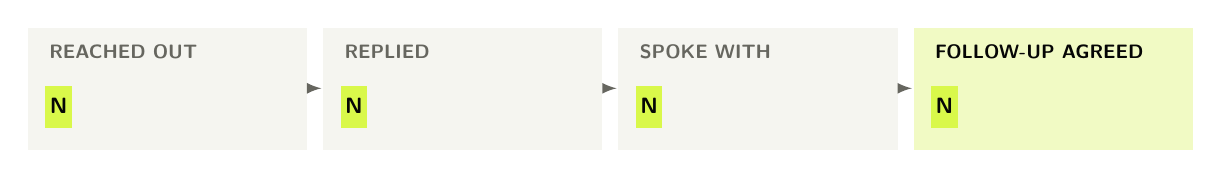
\begin{tikzpicture}[x=1cm,y=1cm,font=\sffamily]
  \def\stage#1#2#3#4{%
    \fill[#3] (#1,0) rectangle ++(3.55,1.55);
    \node[anchor=north west,font=\sffamily\scriptsize\bfseries,text=#4] at (#1+0.15,1.45) {#2};}
  \stage{0}{REACHED OUT}{paper}{muted}
  \stage{3.75}{REPLIED}{paper}{muted}
  \stage{7.5}{SPOKE WITH}{paper}{muted}
  \stage{11.25}{FOLLOW-UP AGREED}{glowsoft}{night}
  \foreach \x in {0,3.75,7.5,11.25}{
    \node[anchor=south west] at (\x+0.1,0.15) {\fillin{N}};}
  \foreach \x in {3.55,7.3,11.05}{
    \draw[-{latex},muted,line width=0.8pt] (\x+0.02,0.78) -- (\x+0.18,0.78);}
\end{tikzpicture}
\end{center}
\src{``Follow-up agreed'' counts people who asked to be told when Firefly launches, or agreed to a second conversation or a pilot. Response rate = replied / reached = \fillin{\%}.}

\subsection{Channels}
{\small
\begin{tabularx}{\linewidth}{@{}>{\raggedright\arraybackslash}X >{\centering\arraybackslash}p{0.72in} >{\centering\arraybackslash}p{0.72in} >{\centering\arraybackslash}p{0.72in} >{\raggedright\arraybackslash}p{1.55in}@{}}
\toprule
\colhead{Channel} & \colhead{Reached} & \colhead{Replied} & \colhead{Spoke} & \colhead{How}\\
\midrule
Co-op cohort and workplace & \fillin{N} & \fillin{N} & \fillin{N} & \fillin{DM, in person}\\
Newcomer Meetup groups (2) & \fillin{N} & \fillin{N} & \fillin{N} & \fillin{at events}\\
Run clubs and walking groups & \fillin{N} & \fillin{N} & \fillin{N} & \fillin{after the run}\\
r/vancouver, r/askvan & \fillin{N} & \fillin{N} & \fillin{N} & \fillin{post + DMs}\\
University newcomer and international societies & \fillin{N} & \fillin{N} & \fillin{N} & \fillin{email}\\
Personal network and LinkedIn & \fillin{N} & \fillin{N} & \fillin{N} & \fillin{DM}\\
\midrule
\textbf{Total} & \fillin{N} & \fillin{N} & \fillin{N} & \\
\bottomrule
\end{tabularx}}

\subsection{Conversation log}
One row per conversation. Participants are anonymised as P01, P02 and so on. The key that links an ID to a person is kept offline and is not part of this document.\par
{\small
\begin{longtable}{@{}>{\sffamily\bfseries}p{0.42in} p{0.78in} p{1.05in} p{0.62in} >{\raggedright\arraybackslash}p{2.55in}@{}}
\toprule
\colhead{ID} & \colhead{Date} & \colhead{Profile} & \colhead{Format} & \colhead{Strongest signal, in their words}\\
\midrule
\endhead
P01 & \fillin{2026-11-\_\_} & \fillin{co-op, 3 mo.} & \fillin{call, 25m} & \fillin{verbatim quote}\\
P02 & \fillin{2026-11-\_\_} & \fillin{new grad, 6 mo.} & \fillin{in person} & \fillin{verbatim quote}\\
P03 & \fillin{2026-11-\_\_} & \fillin{relocated for work} & \fillin{video} & \fillin{verbatim quote}\\
\multicolumn{5}{@{}l}{\src{Add a row for every conversation, including the ones that did not support the thesis.}}\\
\bottomrule
\end{longtable}}

\subsection{Organizers mapped}
Seven Vancouver organizers run recurring events that newcomers attend. Four of them were started by people who moved here and found it hard to make friends. These are prospects we have mapped. None is a partner.\par
{\small
\begin{tabularx}{\linewidth}{@{}>{\raggedright\arraybackslash}p{2.1in} >{\raggedright\arraybackslash}X >{\raggedright\arraybackslash}p{1.35in}@{}}
\toprule
\colhead{Organizer} & \colhead{Format and reported size (as published)} & \colhead{Outreach status}\\
\midrule
Mondays Run Club & Weekly social run, 150+ (VanMag, Feb 2025) & \fillin{status}\\
VanCity Girls Who Walk & Weekly walk, 6 $\to$ 70--200 (Daily Hive, Jul 2024) & \fillin{status}\\
We Should Be Friends & Social club; 100+ at first meetup (VanMag, May 2025) & \fillin{status}\\
Lumi & Newcomer social club; 30 per event, 1,000+ participants (BCIT News, Oct 2026) & \fillin{status}\\
Let's Adventure Vancouver & Social and outdoor group; size not verified & \fillin{status}\\
VanCity Newcomers (20s--30s) & Meetup, 1--2 a month; 5,387 members & \fillin{status}\\
Are you new in Vancouver? & Meetup; 7,234 members & \fillin{status}\\
\bottomrule
\end{tabularx}}
\src{Member counts from the Meetup group pages as retrieved on 15 November 2026. Status: not contacted, contacted, replied, spoke, or committed.}

\subsection{Desk research before the first conversation}
Before any conversations, we reviewed 15 published sources to know what to listen for: two Vancouver Foundation surveys ($n \approx 3{,}800$ each), Statistics Canada's 2025 Survey on Social Connections, and press and first-person accounts from 2017 to 2026 (full list in Appendix C). These are secondary sources. Some of them repeat the same interviews, so we treat them as hypotheses to test, not as proof.\ \desk

% ------------------------------ EVIDENCE ------------------------------
\subsection{Evidence of outreach}
Screenshots are redacted following Appendix B: names, handles, photos, phone numbers, emails and employers are covered with solid blocks. Timestamps and message text that matter are left visible.

\exhibit{a-outreach-message.png}{Outreach message as sent}{The first message, with the recipient redacted. One per channel if the wording differed.}{1.55in}
\exhibit{b-reply-thread.png}{A reply thread}{A redacted DM or email thread where someone describes the problem in their own words.}{1.55in}
\exhibit{c-call-log.png}{Call log}{A calendar or call history showing dates and durations of conversations, with names blurred.}{1.4in}
\exhibit{d-notes-excerpt.png}{Interview notes excerpt}{One page of notes from one conversation, with the participant shown as P\_\_.}{1.4in}

% ------------------------------ 3. PAIN -------------------------------
\section{The main pain point}

\lede{People meet at events. They don't meet again. The leak is at the second meeting, not at the top of the funnel.}

\subsection{Where it leaks}
One Vancouver resident tracked a year of trying to make friends. The pattern holds at every step: plenty of chances to meet people, many first conversations, and almost nobody she still sees.\ \desk

\begin{center}
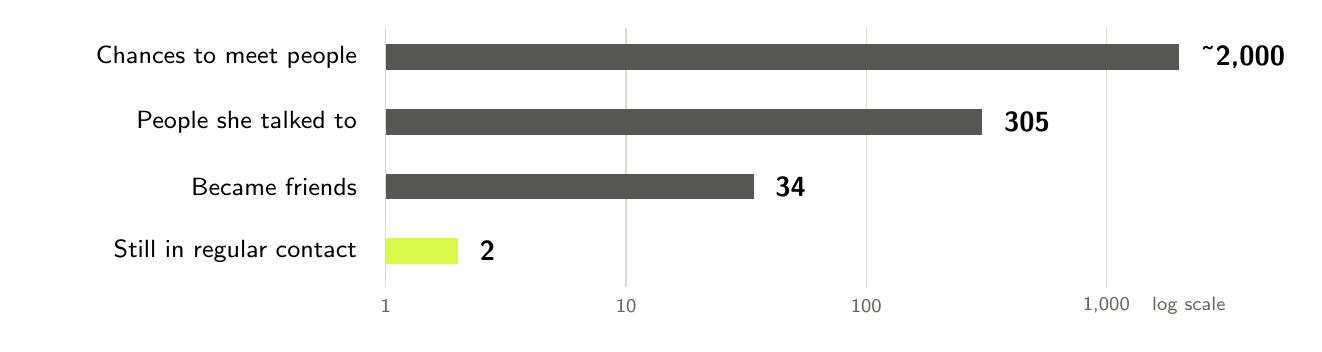
\begin{tikzpicture}[x=3.05cm,y=0.82cm,font=\sffamily\small]
  % log axis ticks
  \foreach \p/\lab in {0/1,1/10,2/100,3/{1,000}}{
    \draw[hair] (\p,0.45) -- (\p,-3.55);
    \node[font=\sffamily\scriptsize,text=muted] at (\p,-3.85) {\lab};}
  \foreach \y/\v/\lab/\col/\txt in {
      0/3.301/{Chances to meet people}/{ink!72}/{\textasciitilde2,000},
      -1/2.484/{People she talked to}/{ink!72}/305,
      -2/1.531/{Became friends}/{ink!72}/34,
      -3/0.301/{Still in regular contact}/glow/2}{
    \fill[\col] (0,\y-0.2) rectangle (\v,\y+0.2);
    \node[anchor=east,text width=1.6in,align=right] at (-0.08,\y) {\lab};
    \node[anchor=west,font=\sffamily\bfseries] at (\v+0.05,\y) {\txt};}
  \node[anchor=west,font=\sffamily\scriptsize,text=muted] at (3.15,-3.85) {log scale};
\end{tikzpicture}
\end{center}
\src{Zetta H., self-tracked year, reported by Daily Hive, 22 January 2025. One person's account, not a population rate. Counts as reported; not independently re-verified.}

\subsection{How often it came up}
Theme counts in the desk sources are tallies of which of the 15 source notes mention a theme. They were not formally coded, and repeated coverage of the same interview is not independent confirmation. The interview column is the one that counts.

\begin{center}
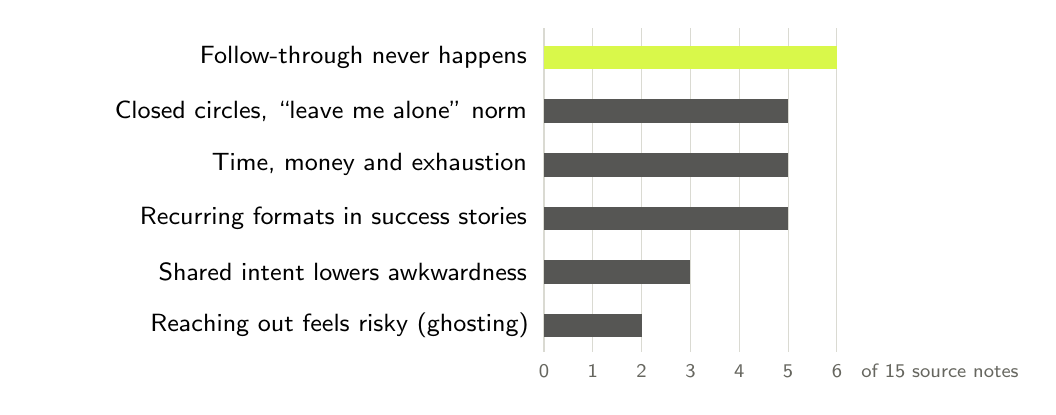
\begin{tikzpicture}[x=0.62cm,y=0.68cm,font=\sffamily\small]
  \foreach \i in {0,...,6}{\draw[hair] (\i,0.55) -- (\i,-5.5);
    \node[font=\sffamily\scriptsize,text=muted] at (\i,-5.85) {\i};}
  \foreach \y/\v/\lab/\col in {
      0/6/{Follow-through never happens}/glow,
      -1/5/{Closed circles, ``leave me alone'' norm}/{ink!72},
      -2/5/{Time, money and exhaustion}/{ink!72},
      -3/5/{Recurring formats in success stories}/{ink!72},
      -4/3/{Shared intent lowers awkwardness}/{ink!72},
      -5/2/{Reaching out feels risky (ghosting)}/{ink!72}}{
    \fill[\col] (0,\y-0.22) rectangle (\v,\y+0.22);
    \node[anchor=east,text width=2.45in,align=right] at (-0.15,\y) {\lab};}
  \node[anchor=west,font=\sffamily\scriptsize,text=muted] at (6.3,-5.85) {of 15 source notes};
\end{tikzpicture}
\end{center}

{\small
\begin{tabularx}{\linewidth}{@{}>{\raggedright\arraybackslash}X >{\centering\arraybackslash}p{1.0in} >{\centering\arraybackslash}p{1.25in} >{\centering\arraybackslash}p{1.0in}@{}}
\toprule
\colhead{Theme} & \colhead{Desk (of 15)} & \colhead{Conversations} & \colhead{Unprompted}\\
\midrule
\textbf{Follow-through never happens} & 6 & \fillin{\_\_ of N} & \fillin{\_\_ of N}\\
Closed circles & 5 & \fillin{\_\_ of N} & \fillin{\_\_ of N}\\
Time, money and exhaustion & 5 & \fillin{\_\_ of N} & \fillin{\_\_ of N}\\
Recurring formats in success stories & 5 & \fillin{\_\_ of N} & \fillin{\_\_ of N}\\
Shared intent lowers awkwardness & 3 & \fillin{\_\_ of N} & \fillin{\_\_ of N}\\
Reaching out feels risky & 2 & \fillin{\_\_ of N} & \fillin{\_\_ of N}\\
\bottomrule
\end{tabularx}}
\src{``Unprompted'' means the person raised it before we asked about it, which is the stronger signal. Count each person once per theme.}

\subsection{What it costs them}
\begin{points}
\item \textbf{Effort that doesn't pay off.} Each conversation that goes nowhere makes the next attempt harder. One newcomer on a forum said they were ``ghosted both times'' and stopped trying.\ \desk
\item \textbf{Time and money spent anyway.} Social clubs report \$15--20 per hangout (BCIT News, 2026). Time alone more than wanted rises from 23\% of all residents to 47\% of households under \$20K (Vancouver Foundation, 2017).\ \desk
\item \textbf{Staying virtual.} 24\% of Canadians whose friendships were virtual-only felt lonely often or always, against 15\% with in-person contact. That is an association, not proof that in-person contact causes the difference (Statistics Canada, 2025).\ \desk
\item \textbf{Leaving.} The founder of We Should Be Friends says some people who commented on her TikTok ``had to leave because it was so hard to meet people'' (VanMag, 2025).\ \desk
\item In our conversations: \fillin{the most concrete cost a participant described, with ID}.\ \firstparty
\end{points}

\pullquote{If you meet someone you connect with, don't just swap numbers --- make a plan to hang out within the next two weeks.}{Katrina Martin, founder of We Should Be Friends (Vancouver Magazine, May 2025). Her rule is the behaviour Firefly is designed to make easy.}

\pullquote{\fillin{The best verbatim quote from your own conversations}}{P\_\_, \fillin{profile, months in Vancouver}}

\subsection{Counter-evidence}
Most of the published evidence supports the problem, but not all of it, and we kept the parts that don't:
\begin{points}
\item Some newcomers say the ``Vancouver Freeze'' is a myth if you put in the effort (Narcity thread, 2022). A friendship coach warns the label can become an excuse.
\item An expert at Douglas College calls urban loneliness ``not just a Vancouver problem'' (2025). We agree and don't claim Vancouver is uniquely lonely.
\item The 2017 survey found frequent loneliness ``lower than expected'' (14\%), even though about half of respondents find it hard to make friends. The problem is making friends, not general unhappiness.
\item From our conversations: \fillin{who did not have this problem, and why}.\ \firstparty
\end{points}

% ------------------------------ 4. DECISION ---------------------------
\section{What we decided to build and test}

\lede{Launch with what helps one person on day one: an easy onboarding and a short personal feed of events. Then build the social layer for the second meeting on top of it.}

\subsection{From evidence to decisions}
{\small
\begin{longtable}{@{}>{\raggedright\arraybackslash}p{1.85in} >{\raggedright\arraybackslash}p{2.35in} >{\raggedright\arraybackslash}p{1.6in}@{}}
\toprule
\colhead{What we learned} & \colhead{What we decided} & \colhead{When}\\
\midrule
\endhead
Events aren't scarce; follow-through is. & The long-term product is repeat meetings with the same people. North star: share of new connections who meet again within 21 days. & Next phase \target\\
Every social app dies of cold start. & Launch scope: two-minute onboarding and a personal event feed, useful before any network exists. & Launch (being built)\\
Event platforms have closed their search APIs (Eventbrite 2020; Luma and Meetup gated). & Events are found by AI-assisted web search in nightly batches per category and area, then checked against each event's own page. No personal data goes to the model. & Launch\\
Cost comes up again and again. & Budget preference in onboarding; free and under-\$20 events by default. & Launch\\
Recurring formats appear in the success stories. & Rank recurring series first, so the same faces come back. & Launch\\
Shared intent lowers awkwardness; closed circles are hard to join. & Small groups for the same event, with a set meeting point, so nobody has to break into a circle. & Next phase\\
Ghosting makes people stop trying. & Picks stay private and mutual. There is never a ``someone liked you'' prompt. & Next phase\\
Showing ``who is here'' can put people at risk. & No location data, ever. The going list is visible only to its owner and deleted after the event. & Built into the design\\
\bottomrule
\end{longtable}}

\subsection{What we chose not to build}
\begin{points}
\item \textbf{A swipe or people-browsing app.} People meet at events they chose, not in a catalogue of strangers.
\item \textbf{Another event platform.} Firefly sits on top of the city's existing events and links out to each event's own page.
\item \textbf{Chat as the product.} Chat only helps arrange the next meeting.
\item \textbf{Hosts at launch.} Organizers are a later channel; attendees come first.
\end{points}

\subsection{What changed because of our conversations}
\begin{callout}{Changes made after talking to people}
\fillin{What the conversations changed}: \fillin{e.g.\ a feature cut, a new segment, a re-ranked priority}.\ \firstparty\par
\fillin{A belief the conversations contradicted, and what we did about it}.\ \firstparty
\end{callout}

\subsection{How we'll know it's working}
{\small
\begin{tabularx}{\linewidth}{@{}>{\raggedright\arraybackslash}X >{\centering\arraybackslash}p{1.15in} >{\raggedright\arraybackslash}p{2.35in}@{}}
\toprule
\colhead{Pilot measure} & \colhead{Target} & \colhead{If we miss it (proposed)}\\
\midrule
Onboarding completion (start $\to$ first feed) & 80\% or more & Cut onboarding questions until it holds.\\
Median time to first feed & Under 2 minutes & Same as above.\\
Listings with a wrong time, place or dead link & Under 2\% & Pause new categories; fix the pipeline.\\
Confirmed ``going'' $\to$ ``I went'' & Set after launch & Interview the people who didn't go.\\
North star: meet again within 21 days & Set in the next phase & This is the thesis: revisit it if the number doesn't move.\\
\bottomrule
\end{tabularx}}
\src{All targets are proposals in the launch spec (workflow/v4-user-flow.md). No pilot has run yet. \target}

% ------------------------------ 5. DEMAND -----------------------------
\section{Evidence of demand}

\lede{Firefly is pre-launch. We are counting signups and commitments only when they are real.}

\subsection{Signals for Firefly itself}
\vspace{2pt}
\begin{minipage}[t]{0.235\linewidth}\stat{\fillin[\LARGE]{N}}{waitlist sign-ups}{since \fillin{date}; via \fillin{channel}}\end{minipage}\hfill
\begin{minipage}[t]{0.235\linewidth}\stat{\fillin[\LARGE]{N}}{pilot commitments (named, dated)}{people who agreed to test it}\end{minipage}\hfill
\begin{minipage}[t]{0.235\linewidth}\stat{\fillin[\LARGE]{N}}{organizer letters of intent}{of 7 mapped organizers}\end{minipage}\hfill
\begin{minipage}[t]{0.235\linewidth}\stat{\fillin[\LARGE]{N}}{intros offered}{people who referred someone else}\end{minipage}

\vspace{8pt}
\exhibit{e-waitlist.png}{Waitlist or sign-up records}{A redacted export or dashboard count with the date visible. Emails masked as a\textbullet\textbullet\textbullet@\textbullet\textbullet\textbullet.}{1.35in}
\exhibit{f-commitment.png}{A pilot commitment or letter of intent}{A redacted message or signed letter from a participant or organizer committing to a dated pilot.}{1.35in}

\subsection{Signals for the category}
These figures come from third parties. They show that people turn up to social events in Vancouver. They are not evidence that people will use Firefly.\ \desk\par
{\small
\begin{tabularx}{\linewidth}{@{}>{\sffamily\bfseries}p{1.0in} X >{\raggedright\arraybackslash}p{1.7in}@{}}
\toprule
\colhead{Figure} & \colhead{What it shows} & \colhead{Source}\\
\midrule
150+ & A weekly social run started by a newcomer from Toronto & Vancouver Magazine, Feb 2025\\
6 $\to$ 70--200 & A free weekly women's walk, grown from six people & Daily Hive, Jul 2024\\
1,000+ & Participants in a newcomer social club that caps events at 30 & BCIT News, Oct 2026\\
5,387 / 7,234 & Members of two Vancouver newcomer Meetup groups & Meetup pages, retrieved 15 Nov 2026\\
\bottomrule
\end{tabularx}}

\begin{callout}[dusk]{What this proves, and what it doesn't}
\textbf{It shows:} people already go to social events in Vancouver, many organizers started their clubs because they were newcomers who couldn't find friends, and surveys show a large share of young adults and newcomers find it hard to make new friends.\par
\textbf{It doesn't show yet:} that people will use Firefly, come back to the feed every week, or meet the same people again. The next 30 days of conversations and the pilot are there to find out.
\end{callout}

% ------------------------------ APPENDICES ----------------------------
\newpage
\appendix
\renewcommand{\thesection}{\Alph{section}}
\makeatletter
\renewcommand{\@seccntformat}[1]{%
  \ifstrequal{#1}{section}{{\color{duskdeep}\sffamily\bfseries Appendix \thesection}\hspace{0.75em}}{%
  {\color{muted}\csname the#1\endcsname}\hspace{0.6em}}}
\makeatother

\section{Conversation guide}
Built on \emph{The Mom Test} (Fitzpatrick) and YC's ``How to Talk to Users'': ask about past behaviour, not opinions about the idea. Firefly is not mentioned until the last five minutes, if at all.
\begin{steps}
\item How long have you been in Vancouver, and what brought you here?
\item Tell me about the last event you went to. How did you find it? Who did you go with?
\item Did you meet anyone there? What happened next?
\item When did you last see someone a second time after meeting them at an event? How did that come about?
\item What's the hardest part about meeting people here? (YC's standard question.)
\item What have you already tried? Apps, clubs, Meetup, Reddit? What happened, and what did you stop using?
\item What did that cost you in time or money?
\item If you could change one thing about it, what would it be?
\item Who else should I talk to?
\end{steps}

\section{Redaction protocol}
\begin{points}
\item Cover every name, handle, profile photo, phone number, email address, employer, school and street address with a \textbf{solid black block}. Don't blur or pixelate: both can be reversed.
\item Keep dates, durations, counts and the message text that carries the evidence visible.
\item Refer to people by participant ID (P01\ldots) only. Keep the key that links IDs to people offline and out of the repository.
\item Re-export the redacted image as a new PNG, so the original layers and metadata aren't carried over, and check for names left in tab titles, notification banners and reply previews.
\item Ask participants for consent before quoting them, even anonymously. Drop any quote that could identify someone in a small community.
\end{points}

\section{Source ledger}
Reviewed 15 November 2026. Several press sources blocked automated retrieval; their figures and quotes are as reported and are marked in the repository's research notes.
{\footnotesize
\begin{longtable}{@{}>{\raggedright\arraybackslash}p{2.0in} >{\raggedright\arraybackslash}p{0.85in} >{\raggedright\arraybackslash}p{3.1in}@{}}
\toprule
\colhead{Source} & \colhead{Date} & \colhead{Used for}\\
\midrule
\endhead
Vancouver Foundation, \emph{Connect \& Engage} ($n$ = 3,785) & 2017 & 67\% / 60\% difficulty making friends; 14\% often lonely; 23\% / 47\% time alone\\
Vancouver Foundation, \emph{Connections and Engagement} ($n$ = 3,841) & 2012 & 50\% of people in Canada under five years\\
Statistics Canada, \emph{Disconnect to reconnect?} & Oct 2025 & 24\% vs.\ 15\% loneliness; recent immigrants 16\% vs.\ 8\% virtual-only\\
Daily Hive, a resident's year of tracking & Jan 2025 & $\sim$2,000 $\to$ 305 $\to$ 34 $\to$ 2\\
CBC News, 30 activities in a month & Jan 2025 & Closed circles; meeting people ``like a job interview''\\
Vancouver Magazine, Mondays Run Club & Feb 2025 & 150+ weekly; founder was a newcomer\\
Vancouver Magazine, We Should Be Friends & May 2025 & Two-week rule; people leaving the city\\
BCIT News, Lumi and social clubs & Oct 2026 & \$15--20 per hangout; 1,000+ participants\\
Daily Hive, VanCity Girls Who Walk & Jul 2024 & Growth from 6 to 70--200\\
Douglas College, Ask an Expert & Jul 2025 & Counter-evidence: not just Vancouver\\
John Zada, ``Vancouver the Lonely'' & May / Sep 2026 & ``Leave me alone'' norm\\
Violet Myles, ``The loneliest city in Canada'' & Oct 2023 & Closed circles, cost\\
Emi Namoro, SFU student project & Undated & Shared intent; exhaustion\\
Narcity, Daily Hive, Reddit threads & 2021--2025 & Ghosting; counter-evidence\\
UBC MHAC, ``Isolated and international'' & Nov 2017 & Proximity and repeated contact\\
\bottomrule
\end{longtable}}

\end{document}
